
\chapter{Week6}

\section{Tuesday}\index{week6_Tuesday_lecture}
\subsection{Summary of previous weeks}
In the first two weeks, we have learnt how to solve linear system of equations $\bm{Ax}=\bm b$. To understand this equation better, we learn the definition for matrices and vector space. The columns of matrix product $\bm{Ax}$ are the linear combination of columns of $\bm{A}$.
\subsubsection{Determinants}
Then we learnt how to describle the \emph{quantity of a matrix}--determinant. The determinant of a square matrix is a single number. This number contains an amazing amount of information about the matrix. There are three main points about determinant:
\begin{itemize}
\item
\textit{Determinants is related to invertibility, rank, eigenvalue, PSD$,\dots$}
\item
$\det(\bm{AB})=\det(\bm A)\det(\bm B).$
\item
\textit{The square matrix $\bm A$ is invertible} if and only if $\det(\bm A)\ne 0.$
\end{itemize}

\subsubsection{Linear Transformation}

Linear transfromation is another important topic. The matrix multiplication $T(\bm v)=\bm{Av}$ is essentially a linear transformation. If we consider a vector as a point in vector space, then \textit{the linear transformation allows movements of point in the space}. It ``transforms'' vector $\bm v$ to another vector $\bm{Av}$.

In the view of linear transformation, we can understand $\det(\bm{AB})=\det(\bm A)\det(\bm B)$ better:
\[
\det(\bm A)=\text{Volumn of $\bm{Ak}$, where $\bm k$ is a unit cube.}
\]

If we transform the unit cube $\bm k$ by $\bm A$ secondly by $\bm B$, actually, it has the same effect of transforming $\bm k$ directly by the matrix $\bm{BA}$.
\begin{figure}[H]
\centering
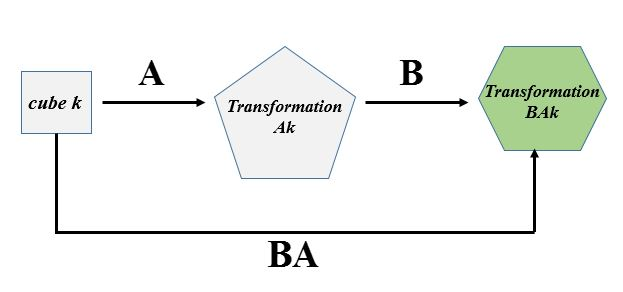
\includegraphics[width=10cm]{week6/determinant}
\caption{Transformation of a vector by $\bm A$, then by $\bm B$ has the same effect by $\bm{BA}$.}
\end{figure}
If we denote $\det(\cdot)$ as the volumn of a graph, since we find that the volumn of $\bm B(\bm{Ak})$ is exactly the same as $(\bm{BA})\bm k$, consequently $\det(\bm B)\det(\bm A)=\det(\bm{BA})$.

Moreover, $\det(\bm A)=0\Longleftrightarrow
\text{Volumn of $\bm{Ak}=0$}\Longleftrightarrow
\dim(\bm{Ak})=0.$

Cramer's Rule also has geometric meaning, which will not be talked in this lecture. (In big data age, people will not use cramer's rule frequently due to its high computing complexity.)

Linear transformation has a matrix representation form under certain basis. \emph{How to transform one basis into another basis?} We use \textit{similar matrices} as the matrix representation, which will be studied in next lecture.
\subsubsection{Orthogonality}
Why we learn orthogonality? It has two motivations:
\begin{enumerate}
\item
Linear independence between vectors
$\Longleftrightarrow\text{Angle}\ne0\degree.$

Similarly, we are interested in the case which the angle is $90$ degrees:
\[
\mbox{orthogonal}\Longleftrightarrow
\mbox{Angle}=90\degree
\]
\item
Solving least squares problem more efficiently.

In pratical, suppose we are given two kinds of data, i.e., 
input: $x =$age of propellant and output: $y = $shear strength. Our data contains $S=\{(x_1,y_1),\dots,(x_{n},y_{n})\}$, $n=20$ samples. Our goal is to find a best line that fit the data:
\begin{figure}[H]
\centering
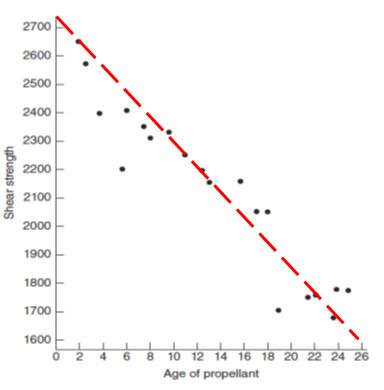
\includegraphics[width=5cm]{week6/regression}
\caption{The relationship between $x$ and $y$.}
\end{figure}
In other words, we want to find $\bm x$ s.t.
\[
    (\tikzmark{identity}{$\bm A$}\tikzmark[red]{G}{$\bm x$}
    \approx\tikzmark[purple]{C}{$\bm b$})
\]
\begin{tikzpicture}[overlay, remember picture,node distance =1.5cm]
    \node (identitydescr) [below left=of identity ]{age};
    \draw[,->,thick] (identitydescr) to [in=-90,out=90] (identity);
    \node[red] (Gdescr) [below =of G]{coefficient};
    \draw[red,->,thick] (Gdescr) to [in=-90,out=90] (G);
    
    \node[purple] (Cdescr) [below right =of C]{strength};
    \draw[purple,->,thick] (Cdescr) to [in=-90,out=90] (C.south);
\end{tikzpicture}

where 
\[
\begin{array}{ll}
\bm A=\begin{bmatrix}
1&x_1\\
1&x_2\\
\vdots&\vdots\\
1&x_{n}
\end{bmatrix}
&
\bm b=\begin{bmatrix}
y_1\\\vdots\\y_n
\end{bmatrix}
\end{array}
\]

More generally, our goal is to solve the least square problem given by:
\[
\min_{\bm x\in\mathbb{R}^{n}}\|\bm{Ax}-\bm b\|^2
\]
where $\bm b\in\mathbb{R}^{m},\bm A\in\mathbb{R}^{m\times n}$.
\begin{itemize}
\item
If $\bm b\in\mathcal{C}(\bm A)$, this optimization problem is converted into finding the solution to equation $\bm{Ax}=\bm b$.
\item
Otherwise, we want to find the least squares solution $\bm x^*$, which must satisfy
\[
\frac{\partial }{\partial \bm x^*}\|\bm{Ax}-\bm b\|^2=\bm 0\implies\bm A\trans\bm A\bm x^*=\bm A\trans\bm b.\qquad\text{(\emph{normal equation.})}
\]
\end{itemize}
This opotimization problem also has geometric meaning. We want to find a solution $\bm x^*$ such that $\bm A\bm x^*$ best approximates the vector $\bm b$, i.e., $\bm A\bm x^* = \Proj_{\mathcal{C}(\bm A)}(\bm b).$
\begin{figure}[H]
\centering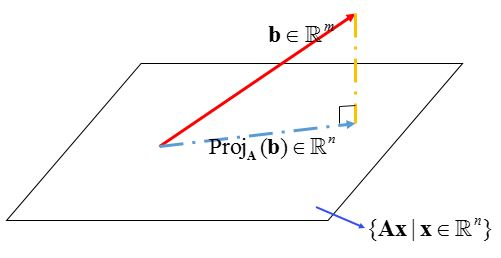
\includegraphics{week6/least_square}
\caption{Least square problem: find $\bm x$ such that $\bm{Ax}=\Proj_{\mathcal{C}(\bm A)}(\bm b).$}
\end{figure}
The expression of the projection $\Proj_{\mathcal{C}(\bm A)}(\bm b)$ is given by:
\[
\Proj_{\mathcal{C}(\bm A)}(\bm b) = \bm A(\bm A\trans\bm A)^{-1}\bm A\trans\bm b.
\]
Therefore, one least squares solution is given by:
\[
\bm x^*=(\bm A\trans\bm A)^{-1}\bm A\trans\bm b.
\]
When $\bm A$ has full column rank, this solution is the unique least squares solution. (verify by yourself)

Moreover, when $\bm A$ is an \emph{orthogonal matrix}, the least squares solution could be computed more efficiently:
\[
\bm x^*=\bm Q\trans\bm b.
\]
\end{enumerate}

\subsection{Eigenvalues and eigenvectors}
\subsubsection{Why do we study eigenvalues and eigenvectors?}
\begin{itemize}
\item
\emph{Motivation 1: }If we consider matrices as the \textit{movements} (linear transformation) for \textit{vectors} in vector space. Then roughly speaking, \textit{eigenvalues} are the \textit{speed} of the movements, \textit{eigenvectors} are the \textit{direction} of the movements
\item
\emph{Motivation 2: }We know that linear transformation has different matrix representation for different basis. But which representation is \emph{simplest} for a linear transformation? This topic gives us answer to this question.
\end{itemize}
When vectors are multiplied by $\bm A$, almost all vectors change direction. If $\bm x$ has the same direction as $\bm{Ax}$, they are called \emph{eigenvectors}.
\[
\begin{array}{lll}
\mbox{\emph{The key equation is}}
&
\bm{Ax}=\lambda\bm x,
&
\emph{The number $\lambda$ is the eigenvalue of $\bm A$.}
\end{array}
\]
\begin{definition}[Eigenvectors and Eigenvalues]
Given a matrix $\bm A\in\mathbb{R}^{n\times n}$ (or $\mathbb{C}^{n\times n}$), our goalis to find a vector $\bm v\in\mathbb{C}^n$ with $\bm v\ne\bm 0$ such that
\begin{equation}\label{Eq:7:1}
\begin{array}{ll}
\bm A\bm v=\lambda\bm v,
&
\mbox{for some $\lambda\in\mathbb{C}$}
\end{array}
\end{equation}
\begin{itemize}
\item
(\ref{Eq:7:1}) is called an \emph{eigenvalue problem} or \emph{eigen-equation}
\item
Let $(\bm v,\lambda)$ be a solution to (\ref{Eq:7:1}), we call
\begin{itemize}
\item
$(\bm v,\lambda)$ an \emph{eigen-pair} of $\bm A$
\item
$\lambda$ an \emph{eigenvalue} of $\bm A$; $\bm v$ an \emph{eigenvector} of $\bm A$ associated with $\lambda$.
\end{itemize}
\end{itemize}
\end{definition}
We illustrate an example of an eigenvalue problem:
\begin{example}
Consider an eigenvalue problem $\bm{Ax}=\lambda\bm x$, where
\[
\begin{array}{ll}
\bm A=\begin{bmatrix}
4&-2\\1&1
\end{bmatrix},
&
\bm x=\begin{bmatrix}
2\\1
\end{bmatrix}
\end{array}
\]

We can verify that
\[
\bm{Ax}=\begin{bmatrix}
6\\3
\end{bmatrix}=3\begin{bmatrix}
2\\1
\end{bmatrix}=3\bm x
\]

Therefore, $\lambda=3$ is the eigenvalue of $\bm A$; $\bm x=\begin{bmatrix}
2\\1
\end{bmatrix}$ is the eigenvector of $\bm A$ associated with $\lambda=3.$
\end{example}
\begin{proposition}
If $(\bm v,\lambda)$ is an eigen-pair of $\bm A$, then $(\alpha\bm v,\lambda)$ is also an eigen-pair for any $\alpha\in\mathbb{C},\alpha\ne0$.
\end{proposition}

\subsubsection{Calculation for eigen-pairs}
How to find eigen-pairs $(\lambda,\bm x)$? In other words, how to solve the nonlinear equation $\bm{Ax}=\lambda\bm x$, where $\lambda$ and $\bm x$ are unknowns? Consider a simpler case. If we can know the eigenvalues $\lambda$, then we can solve the linear system $(\lambda\bm I-\bm A)\bm x=\bm 0$ to get the corresponding eigenvectors.

But how to find eigenvalues? $\bm{Ax}=\lambda\bm x$ has a nonzero solution $\Longleftrightarrow$$(\lambda\bm I-\bm A)\bm x=\bm 0$ has a nonzero solution $\Longleftrightarrow$ $(\lambda\bm I-\bm A)$ is singular $\Longleftrightarrow$$\det(\lambda\bm I-\bm A)=0.$

Therefore, solving the determinant equation gives a way to find eigenvalues:
\begin{proposition}
The number $\lambda$ is the eigenvalue of $\bm A$ if and only if $\lambda\bm I-\bm A$ is singular.
\begin{equation}
\begin{array}{ll}
\mbox{\emph{Equation for the eigenvalues}}
&
\det(\lambda\bm I-\bm A)=0.
\end{array}
\end{equation}
\end{proposition}

\begin{definition}[characteristic polynomial]
Define $P_{\bm A}(\lambda):=\det(\lambda\bm I-\bm A)$. 

Then $P_{\bm A}(\lambda)=\det(\lambda\bm I-\bm A)$ is called the \emph{characteristic polynomial} for the matrix $\bm A$; the equation $\det(\lambda\bm I-\bm A)=0$ is called the \emph{characteristic equation} for the matrix $\bm A$; the set $N(\lambda\bm I-\bm A)$ is called the \emph{eigenspace} associated with $\lambda$.

If $P_{\bm A}(\lambda^{*})=0$, then we say $\lambda^*$ is the root of $P_{\bm A}(\lambda)$.
\end{definition}

The roots of $P_{\bm A}(\lambda)$ are the \emph{eigenvalues} of $\bm A$. $\forall\bm x\in N(\lambda\bm I-\bm A)$ (\textit{eigenspace}) is an eigenvector associated with $\lambda$.

\begin{example}
Find the eigenvalues and eigenvectors of $\bm A=\begin{bmatrix}
3&2\\3&-2
\end{bmatrix}$.\\
\begin{gather*}
\det(\lambda\bm I-\bm A)=\begin{bmatrix}
\lambda -3&-2\\-3&\lambda+2
\end{bmatrix}=0.\\
\implies (\lambda+3)(\lambda-2)-6=0.
\implies \lambda^2-\lambda-12=0.\implies
\lambda_1=4\quad\lambda_2=-3.
\end{gather*}
Eigenvalues of $\bm A$ are $\lambda_1=4\text{ and }\lambda_2=-3.$\\
In order to get eigenvectors, we solve $(\bm A-\lambda\bm I)\bm x=\bm 0$:
\begin{itemize}
\item
For $\lambda_1$, $(\bm A-\lambda_1\bm I)\bm x=\begin{bmatrix}
-1&2\\3&-6
\end{bmatrix}=\bm 0$.
\[
\implies \bm x=\begin{bmatrix}
2x_2\\x_2
\end{bmatrix}=x_2\begin{bmatrix}
2\\1
\end{bmatrix}
\]
Hence any $\alpha\begin{bmatrix}
2&1
\end{bmatrix}\trans$ $(\alpha\ne0)$ is the eigenvector of $\bm A$ associated with $\lambda_1=4.$
\item
For $\lambda_2$, similarly, we derive
\[
\bm x=\begin{bmatrix}
-x_2\\3x_2
\end{bmatrix}=x_2\begin{bmatrix}
-1\\3
\end{bmatrix}
\]
Hence any $\beta\begin{bmatrix}
-1&3
\end{bmatrix}\trans$ $(\beta\ne0)$ is the eigenvector of $\bm A$ associated with $\lambda_2=-3.$
\end{itemize}
\end{example}

\subsubsection{Possible difficulty: how to solve $\det(\lambda\bm I-\bm A)=0$?}
$P_{\bm A}(\lambda)$ is a characteristic polynomial with degree $n$. Actually, we can write $P_{\bm A}(\lambda)$ as:
\[
P_{\bm A}(\lambda)=\lambda^n-a_1\lambda^{n-1}+a_2\lambda^{n-2}-\dots+(-1)^{n}a_n
\]
where $a_i$'s depend on matrix $\bm A$.

When $n$ increases, it's hard to find its roots:
\begin{itemize}
\item
When $n=2,3,4$, solution to $P_{\bm A}(\lambda)=0$ has the \textit{closed form}, which has been proved in $15$th century.
\item
However, when $n\ge5$, the characteristic equation has \textit{no closed form} solution.
\end{itemize}

Although we cannot find closed form solution for large $n$, we want to study whether this characteristic polynomial with degree $n$ has exactly $n$ solutions. Gauss gives us the answer:
\begin{theorem}[Fundamental theorem of algebra]
Every nonzero, single variable, degree $n$ polynomial with \textit{complex coefficients} has \textit{exactly} $n$ complex roots. (Counted with multiplicity.)
\end{theorem}

What's the meaning of \textit{multiplicity?} For example, the polynomial $(x-1)^2$ has one root 1 with multiplicity 2.

\paragraph{Implication}
Hence, every polynomial $f(x)$ could be written as
\begin{align*}
f(x)&=a_nx^n+a_{n-1}x^{n-1}+\dots+a_1x_1+a_0\\
&=a_n(x-x_1)(x-x_2)\dots(x-x_n)
\end{align*}
where $x_i$'s are roots for $f(x)$.

Moreover, \emph{$P_{\lambda}(\bm A)$ has exactly $n$ roots, i.e., $\bm A$ has $n$ eigenvalues.(counted with multiplicity.)}
\begin{remark}
Exact roots are almost impossible to find. But approximate roots (eigenvalues) can be find easily by numerical algorithm.
\end{remark}
\subsection{Products and Sums of Eigenvalue}
\paragraph{The coefficient of the highest order for the characteristic polynomial is 1}
Suppose $P_{\bm A}(\lambda)=\det(\lambda\bm I-\bm A)$ has $n$ roots $\lambda_1,\dots,\lambda_n$, then we obtain:
\begin{equation}
P_{\bm A}(\lambda)=\det(\lambda\bm I-\bm A)=(\lambda-\lambda_1)\dots(\lambda-\lambda_n)
\label{characteristic}
\end{equation}
Why the coefficient for $\lambda^{n}$ is 1 in equation (\ref{characteristic})? If we expand $\det(\lambda\bm I-\bm A)$, we find
\begin{equation}
\det(\lambda\bm I-\bm A)=\begin{vmatrix}
\lambda-a_{11}&-a_{12}&\dots&-a_{nn}\\
-a_{21}&\lambda-a_{22}&\dots&-a_{2n}\\
\vdots&\vdots&\ddots&\vdots\\
-a_{n1}&\dots&\dots&\lambda-a_{nn}
\end{vmatrix},
\label{characteristic_det}
\end{equation}
in which the variable $\lambda$ only appears in diagonal. By expaning  the determinant, the coefficient of highest order is obviously 1.
\paragraph{The sum of eigenvalues equals to the sum of the $n$ diagonal entries of $\bm A$}
In $(\ref{characteristic})$, the coefficient of $\lambda^{n-1}$ is
\[
-(\lambda_1+\lambda_2+\dots+\lambda_n)
\]

In $(\ref{characteristic_det})$, $\lambda^{n-1}$ only appears among $(\lambda-a_{11})(\lambda-a_{22})\dots(\lambda-a_{nn})$, i.e., the coefficient of $\lambda^{n-1}$ is
\[
-(a_{11}+a_{22}+\dots+a_{nn})
\]

Consequently, as $(\ref{characteristic})=(\ref{characteristic_det})$, we obtain
\[
\sum\lambda_i=\text{\emph{trace}}=\sum a_{ii}
\]
The sum of the entries on the main diagonal is called the \emph{trace} of $\bm A$, denoted by $\trace(\bm A)$.
\paragraph{The product of the eigenvalues equals to the determinant of $\bm A$}
If let $\lambda=0$ in $(\ref{characteristic})$, then we obtain $\det(-\bm A)=(-1)^n\lambda_1\lambda_2\dots\lambda_n$. Obviously, $\det(-\bm A)=(-1)^{n}\det(\bm A)$. 

Hence $(-1)^{n}\det(\bm A)=(-1)^n\lambda_1\lambda_2\dots\lambda_n\implies
\det(\bm A)=\lambda_1\lambda_2\dots\lambda_n.$

\begin{theorem}
\emph{\textit{The product of the $n$ eigenvalues equals the determinant of $\bm A$.}}\\
\emph{\textit{The sum of the $n$ eigenvalues equals the sum of the $n$ diagonal entries of $\bm A$.}}
\end{theorem}

\subsection{Application: Page Rank and Web Search}
Google is the largest web search engine in the world. When you enter a keyworld, the \textit{PageRank} algorithm is used by Google to rank the search results of your keyworld.
\begin{figure}[H]
    \begin{minipage}[b]{0.5\textwidth} 
      \centering 
      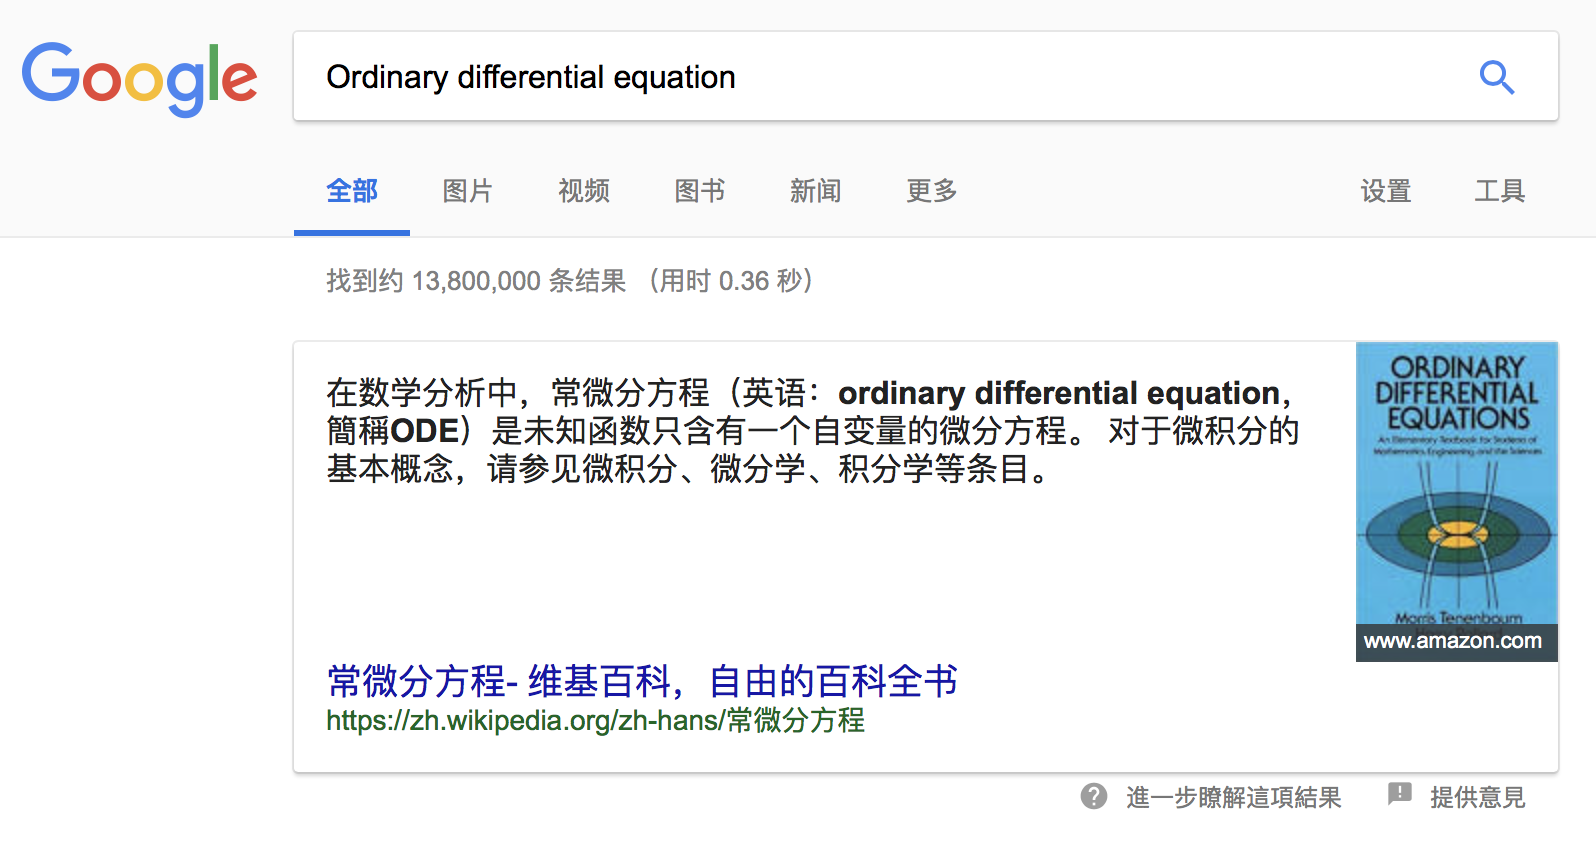
\includegraphics[width=3in]{week6/Fig_1.png} 
      \caption{Google interface}
    \end{minipage}%  
    \begin{minipage}[b]{0.5\textwidth} 
      \centering 
      
\includegraphics[width=3in]{week6/Fig_2.png}
      \caption{PageRank Diagram, source: Wiki}
    \end{minipage}
\end{figure}
To rank the pages with respect to its importance, the idea is to use counts of links of other pages, i.e., if a page is referenced by many many other pages, it must be very important.
\paragraph{PageRank Model} The PageRank model is given as follows:
\begin{equation}
\sum_{j\in\mathcal{L}_i}\frac{v_j}{c_j}=v_i,\quad
i=1,\dots,n,\label{Eq:7:5}
\end{equation}
where $c_j$ is the number of outgoing links from page $j$; $\mathcal{L}_i$ is the set of pages with
a link to page $i$; $v_i$ is the importance score of page $i$. (We skip the procedure for how to construct this model)
\begin{example}
If we assume that there are only four pages in the world, and the diagram below shows the reference situations:
\begin{figure}[H]
\centering
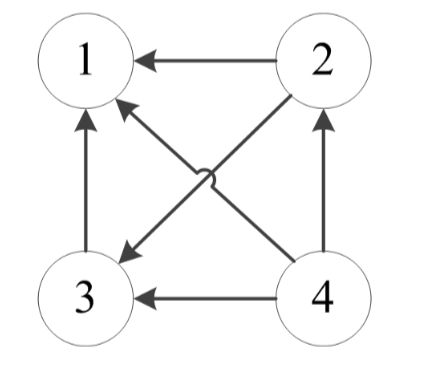
\includegraphics[width=3in]{week6/Fig_3.png}
\caption{Reference situation of these four pages}
\label{fig:7:3}
\end{figure}
Let's consider the $i=3$ case of Eq.(\ref{Eq:7:5}). The set of pages with a link to page $3$ is
\[
\mathcal{L}_3:=\{2,4\}
\]

Next, we find that the number of outgoing links from page $2,4$ are $2,3$ respectively. Hence we build a equation for $i=3$ case:
\[
\frac{v_2}{2}+\frac{v_4}{3}=v_3
\]

Similarly, we could use this procedure to obtain the $i=1,2,3,4$ cases of Eq.(\ref{Eq:7:5}):
\begin{align*}
\frac{1}{2}v_2+v_3+\frac{1}{3}v_4&=v_1\\
\frac{1}{3}v_4&=v_2\\
\frac{1}{2}v_2+\frac{1}{3}v_4&=v_3\\
0&=v_4
\end{align*}
Or equailently, we write the equations above into matrix form:
\[
\underbrace{\begin{bmatrix}
0&\frac{1}{2}&1&\frac{1}{3}\\
0&0&0&\frac{1}{3}\\
0&\frac{1}{2}&0&\frac{1}{3}\\
0&0&0&0
\end{bmatrix}}_{\bm A}\underbrace{\begin{bmatrix}
v_1\\v_2\\v_3\\v_4
\end{bmatrix}}_{\bm v}=\underbrace{\begin{bmatrix}
v_1\\v_2\\v_3\\v_4
\end{bmatrix}}_{\bm v}
\]
\end{example}
\paragraph{PageRank Problem}Our goal is to find the importance score $v_i$, i.e., find a \emph{non-negative} $\bm v$ such that $\bm{Av}=\bm v$. 

In practical, $\bm A$ is extremely large and sparse. To solve such a eigenvalue problem, we want to use the numerical method (power method). The further reading is recommended:
\begin{quotation}
K. Bryan and L. Tanya, “The 25, 000, 000, 000 eigenvector: The linear
algebra behind Google,” SIAM Review, vol. 48, no. 3, pp. 569–581, 2006.
\end{quotation}



